%%%%%%%%%%%%%%%%%%%%%%%%%%%%%%%%%%%%%%%%%%%%%%%%%%%%%%%%%%%%%%%%%%%%%%
% LaTeX Example: Project Report
%
% Source: http://www.howtotex.com
%
% Feel free to distribute this example, but please keep the referral
% to howtotex.com
% Date: March 2011 
% 
%%%%%%%%%%%%%%%%%%%%%%%%%%%%%%%%%%%%%%%%%%%%%%%%%%%%%%%%%%%%%%%%%%%%%%

\documentclass[paper=a4, fontsize=11pt]{scrartcl}
\usepackage[T1]{fontenc}
\usepackage{fourier}

\usepackage[english]{babel}															% English language/hyphenation
\usepackage[protrusion=true,expansion=true]{microtype}	
\usepackage{amsmath,amsfonts,amsthm} % Math packages
\usepackage[pdftex]{graphicx}	
\usepackage{url}
\usepackage{listings}

%%% Custom sectioning
\usepackage{sectsty}
\allsectionsfont{\centering \normalfont\scshape}

%%% Custom headers/footers (fancyhdr package)
\usepackage{fancyhdr}
\pagestyle{fancyplain}
\fancyhead{}											% No page header
\fancyfoot[L]{}											% Empty 
\fancyfoot[C]{}											% Empty
\fancyfoot[R]{\thepage}									% Pagenumbering
\renewcommand{\headrulewidth}{0pt}			% Remove header underlines
\renewcommand{\footrulewidth}{0pt}				% Remove footer underlines
\setlength{\headheight}{13.6pt}

%%% Equation and float numbering
\numberwithin{equation}{section}		% Equationnumbering: section.eq#
\numberwithin{figure}{section}			% Figurenumbering: section.fig#
\numberwithin{table}{section}				% Tablenumbering: section.tab#

%%% Maketitle metadata
\newcommand{\horrule}[1]{\rule{\linewidth}{#1}} 	% Horizontal rule

%%%% stuff for code
\usepackage{color}
 
\definecolor{codegreen}{rgb}{0,0.6,0}
\definecolor{codegray}{rgb}{0.5,0.5,0.5}
\definecolor{codepurple}{rgb}{0.58,0,0.82}
\definecolor{backcolour}{rgb}{0.95,0.95,0.92}
 
\lstdefinestyle{mystyle}{
    backgroundcolor=\color{backcolour},   
    commentstyle=\color{codegreen},
    keywordstyle=\color{magenta},
    numberstyle=\tiny\color{codegray},
    stringstyle=\color{codepurple},
    basicstyle=\footnotesize,
    breakatwhitespace=false,         
    breaklines=true,                 
    captionpos=b,                    
    keepspaces=true,                 
    numbers=left,                    
    numbersep=5pt,                  
    showspaces=false,                
    showstringspaces=false,
    showtabs=false,                  
    tabsize=2
}
\lstset{style=mystyle}
%%%%%%%%%

\title{
		%\vspace{-1in} 	
		\usefont{OT1}{bch}{b}{n}
		\normalfont \normalsize \textsc{ Beam Physics Departments } \\ [25pt]
		\horrule{0.5pt} \\[0.4cm]
		\huge How to use ISYN, a longitudinal tracking code in particle accelerator\\
		\huge Manual
		\horrule{2pt} \\[0.5cm]
}
\author{
		\normalfont 								\normalsize
        Sandra Aumon, Paul G\"orgen\\[-3pt]		\normalsize
        \today
}
\date{}

\begin{document}
\maketitle

\section{how to use ISYN}
\label{howto}

\section{code comparison with beam dynamics: benchmarks}
This section is dedicated to compared Isyn simulation results to the longitudinal beam dynamics theory in very specific and well known scenarii used in accelerators. Most of the cases will be apply to the FAIR-SIS100 and also to the CERN PS machine. The following longitudinal beam simulations will be presented here, the aim being to compare the results of Isyn to the theory and observe the behaviour of the tracking code:
\begin{enumerate}
\item The simple case of a stationary single harmonic bucket, without collective effect.
\item A bunch rotation with a proton beam.
\item Simple acceleration.
\item Acceleration through transition energy.
\item A stationary single harmonic bucket with longitudinal space charge.
\item Acceleration with longitudinal space charge through transition energy.
\end{enumerate}

For each cases, an short description of the interface python main file will be given and explained as well as the theory used to compare with. Then the results of the simulations are shown. Remarks and discussions can be triggered if the  special effects or code artefacts are found.


\subsection{single harmonic stationary bucket}
The case of a simple single harmonic bucket has been simulated in Isyn. The particle coordinates have been generated within an elliptical distribution, and the simulation is done with the SIS-100 beam parameter around injection energy. The particles are tracked with one kick per turn for 50 000 turns, as a first step.

In this paragraph, the namely file \detokenize{Isyn_StationaryBucket_noSc.py} is described.
For this simulation, we need the following imports for Python, 

\begin{lstlisting}[language=Python]

from accelerator.Accelerator import Accelerator
from accelerator.Accelerator_Info import Accelerator_Info
from beamofparticle.Beam import Beam
from radiofrequency.RFcavity import RFcavity
import cProfile # Useful to monitor the time taking by each module of the code. Not mandatory.

\end{lstlisting}

First an Accelerator Python Object is created, as refered in Section~\ref{howto}.

\begin{lstlisting}[language=Python]

#--------------- Declare the Object Accelerator ------------#

sis100 = Accelerator() # here my accelerator is sis100
sis100.setRadius(172.4603) # the machine radius
sis100.gammat = 8.9 # the transition gamma
sis100.bdot = 0.0 # the dB/dt , here zero since no acceleration
sis100.gammadot = 0.0 

sis100.setParameterFilename('sis100') # any comment that you like for your file name in output
sis100.dumpDistributionEveryNturn(1000) # Particle coordinates written into a file every 1000 turns 

\end{lstlisting}

Then a Beam Python Object is created, as refered in Section~\ref{howto}.

\begin{lstlisting}[language=Python]

# --------------- Declare the Object Beam ------------#

beam = Beam() # I create a Beam Object beam
beam.setGamma(5.0) # with an gamma of 5
beam.setRestEnergy(938272046.0)
beam.setCharge(1.0) # Protons are used
beam.setNParticle(100000) # 100k macroparticles will be tracked
beam.parabolicDistribution(0.509, 0.001418, 0.0) # The distribution is chosen Parabolic.

\end{lstlisting}

This part prints some info about the simulation you created. The momentum compaction factor is then given, computed from the Objects beam and sis100.

\begin{lstlisting}[language=Python]

# --------------- Get the Object Accelerator_Info ------------#

info = Accelerator_Info(sis100, beam) 

\end{lstlisting}

Then, a Python Object RFcavity is created to simulate the RF kick given to the particles each turn.
\begin{lstlisting}[language=Python]

# --------------- Declare the Object Rfcavity ------------#

rf = RFcavity(sis100) 
rf.setHarmonic(10) # RF Harmonic
rf.setRFvoltage(60000.0) # the voltage in Volt
rf.setStablePhase(0.0) # the stable phase, here zero.
sis100.addElement(rf) # Add the RF cavity to the beam line.

\end{lstlisting}

Finally, the tracking can start, according to two possibilities. If there an interest to monitor the speed of the code, one can use cProfile in order to see how long each module is taking to perform the computations.

\begin{lstlisting}[language=Python]

# --------------- Tracking ------------#

cProfile.run('sis100.track(beam, 50000)','restats')
import pstats
p = pstats.Stats('restats')
p.sort_stats('cumulative').print_stats(10)

\end{lstlisting}

Or, without time monitoring,

\begin{lstlisting}[language=Python]
# --------------- Tracking ------------#

sis100.track(beam, 50000) 
# Here start the tracking of 100k macroparticles over 50k turns
\end{lstlisting}

\begin{figure}[h!]
  \centering
  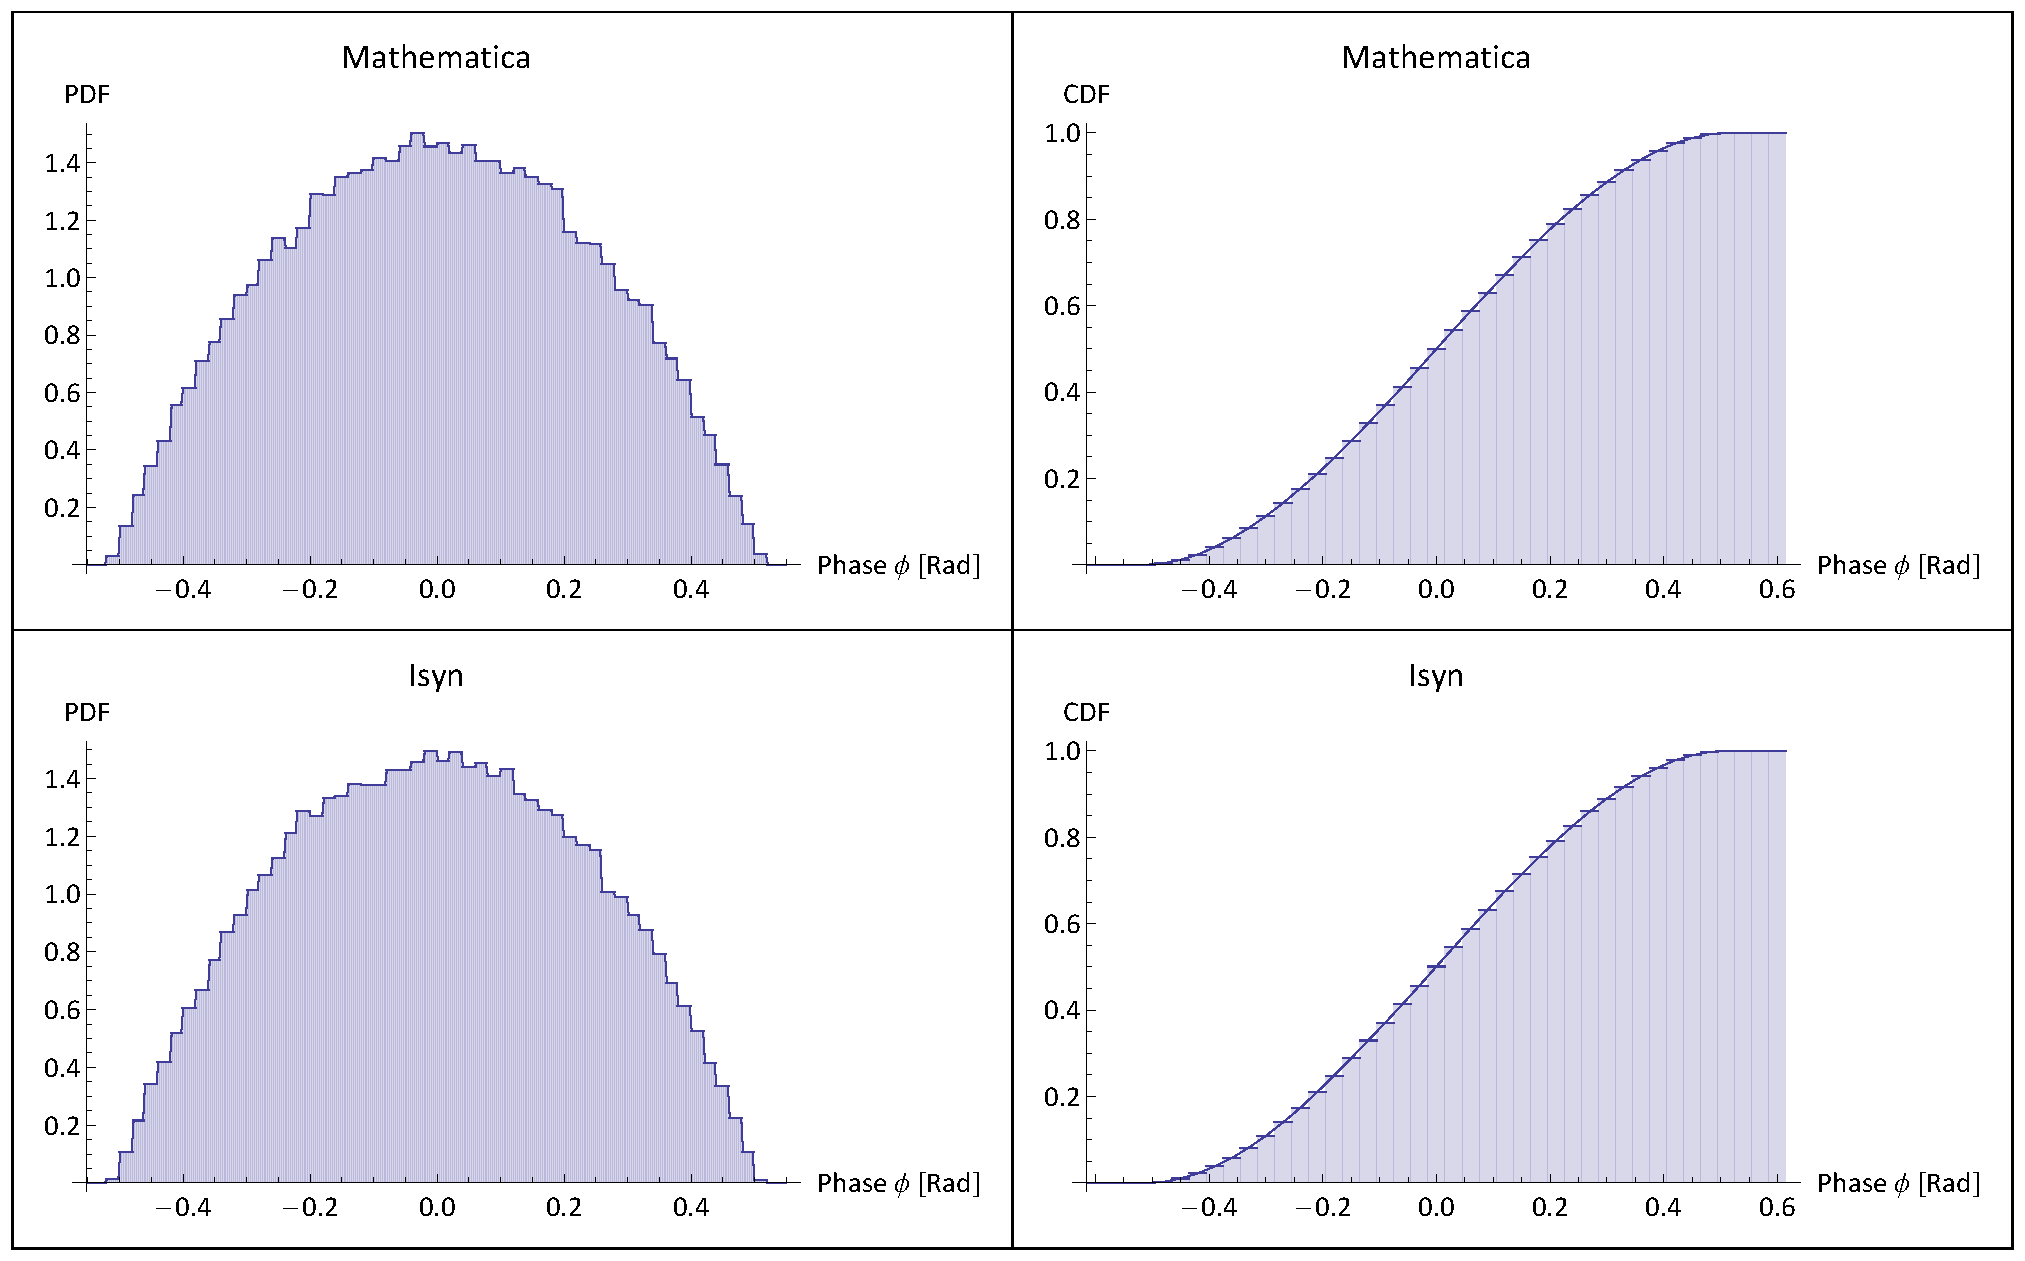
\includegraphics[width=13cm]{benchmarks/pics/FinalCDFplots.pdf}\\
  \caption{CDF .}
\label{fig:rfsetting}
\end{figure}

\begin{figure}[h!]
  \centering
  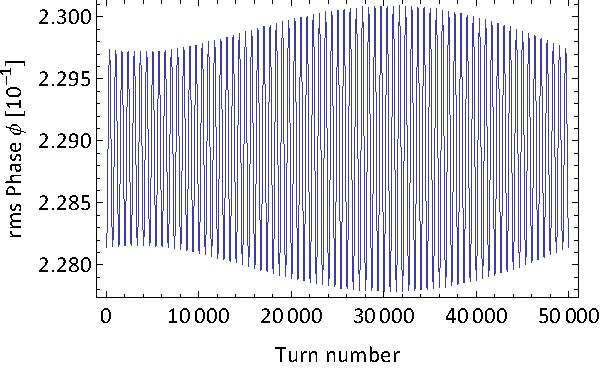
\includegraphics[width=9cm]{benchmarks/pics/StatBucketbl.pdf}\\
  \caption{bunch length.}
\label{fig:rfsetting}
\end{figure}

\begin{figure}[h!]
  \centering
  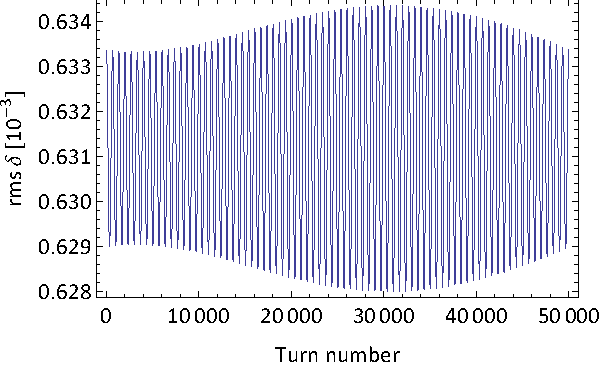
\includegraphics[width=9cm]{benchmarks/pics/StatBucketdelta.pdf}\\
  \caption{delta.}
\label{fig:rfsetting}
\end{figure}








\end{document}